\section{Blockchain}
In diesem Kapitel wird auf die revolutionären Vorteile der Blockchain 
eingegangen, durch die diese Technologie Einzug in den Finanzsektor gewonnen 
hat. Dem werden im Nachgang die einhergehenden Nachteile und Risiken gegenübergestellt. 

\subsection{Aufbau einer Blockchain}
Ein elementarer Grundbaustein einer Blockchain ist die Bildung eines Hashes.
\glqq Eine Hash-Funktion bildet eine beliebig große Menge an Eingabedaten [...] auf eine Zahl von 
fixer Größe ab, den sogenannten Hashwert\grqq{} \cite[p.~6]{fill2020blockchain}.
Die Hash-Funktion erfüllt darüber hinaus drei wichtige Prinzipien.
Das Diffusionsprinzip beschreibt eine deutliche Änderung des Hashwertes bei einem leicht
abgeänderten Eingabewert. Dadurch können unterschiedliche Eingaben sofort erkannt werden.
Das Konfusionsprinzip beschreibt die Eigenschaft, dass vom Hashwert nicht auf den Eingabewert
geschlossen werden kann. Beim Vergleich zweier Hashwerte von Eingaben mit einer minimalen
Änderung kann nichtmal die Position der Abweichung geschlossen werden.
\cite[p.~6ff]{fill2020blockchain} 

Um die Einsatzgebiete für eine Blockchain im Finanzsektor besser zu verstehen,
wird im Folgenden der Aufbau und die Komponenten grob dargestellt.
Im Block 1 wird zuerst jeweils ein Hash H1 und H2 für die Datenpunkte Transaktion 1 
und Transaktion 2 gebildet. Aus diesen Hashes wird dann ein gemeinsamer Hash H12 gebildet, 
der den Block Header 1 darstellt.
Analog zum Block Header 1 wird Block Header 2 erstellt. Zusätzlich enthält dieser eine
Referenz auf den vorigen Block Header 1 und ist somit der Kopf der Kette. Der Block Header 2
kann weiterführend im Block Haeder 3 eines dritten Blocks referenziert werden. 
\ref{fig:BC_Aufbau}
\cite[p.~17f]{fill2020blockchain}

\begin{figure}[h!]
    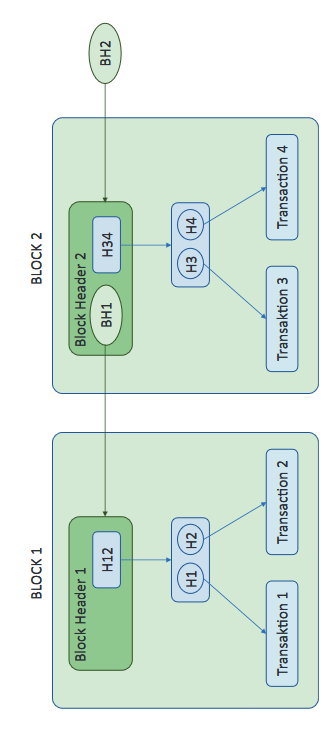
\includegraphics[width=\columnwidth]{BC_Aufbau.png}
    \quelle{\cite[p.~19]{fill2020blockchain}}
    \caption{Aufbau einer Blockchain \cite[p.~19]{fill2020blockchain}}
    \label{fig:BC_Aufbau}
\end{figure}

\subsection{}